\documentclass[dvipdfmx]{jarticle}
\usepackage[dvipdfmx]{graphicx}
\usepackage{mediabb}
\usepackage{yokou}
\usepackage{amsmath}
\usepackage{amsfonts}
\usepackage{array}
\usepackage{multirow}
\usepackage{mathtools}
\usepackage{float}
\usepackage{pdfpages}

%ここからソースコードの表示に関する設定
\usepackage{listings,jlisting}
\lstset{
  basicstyle={\ttfamily},
  identifierstyle={\small},
  commentstyle={\smallitshape},
  keywordstyle={\small\bfseries},
  ndkeywordstyle={\small},
  stringstyle={\small\ttfamily},
  frame={tb},
  breaklines=true,
  columns=[l]{fullflexible},
  numbers=left,
  xrightmargin=0zw,
  xleftmargin=0zw,
  numberstyle={\scriptsize},
  stepnumber=1,
  numbersep=1zw,
  lineskip=-0.5ex
}

\title{WANNにおけるシナプス荷重の調整と活性化関数の慎重な選択}
\author{増田 瑞樹}
%\発表日{2023年 11月 3日}
\学生番号{2031133}
\begin{document}
\maketitle

\section{WANN}
Weight Agnostic Neural Networks(WANN) は,ネットワーク構造を更新することでどんなシナプス荷重に対してもそれなりの精度でタスクを解くことができるようになる.変更するノードは隠れ層からランダムに選択され,現在採用されている活性化関数をのぞいた活性化関数の中から,同等の確率で選択される.また,ネットワークの評価には-2.0, -1.0, -0.5, +0.5, +1.0, +2.0の共有重みを用いた6つの評価の平均を採用している.

\begin{figure}[h]
    \centering
    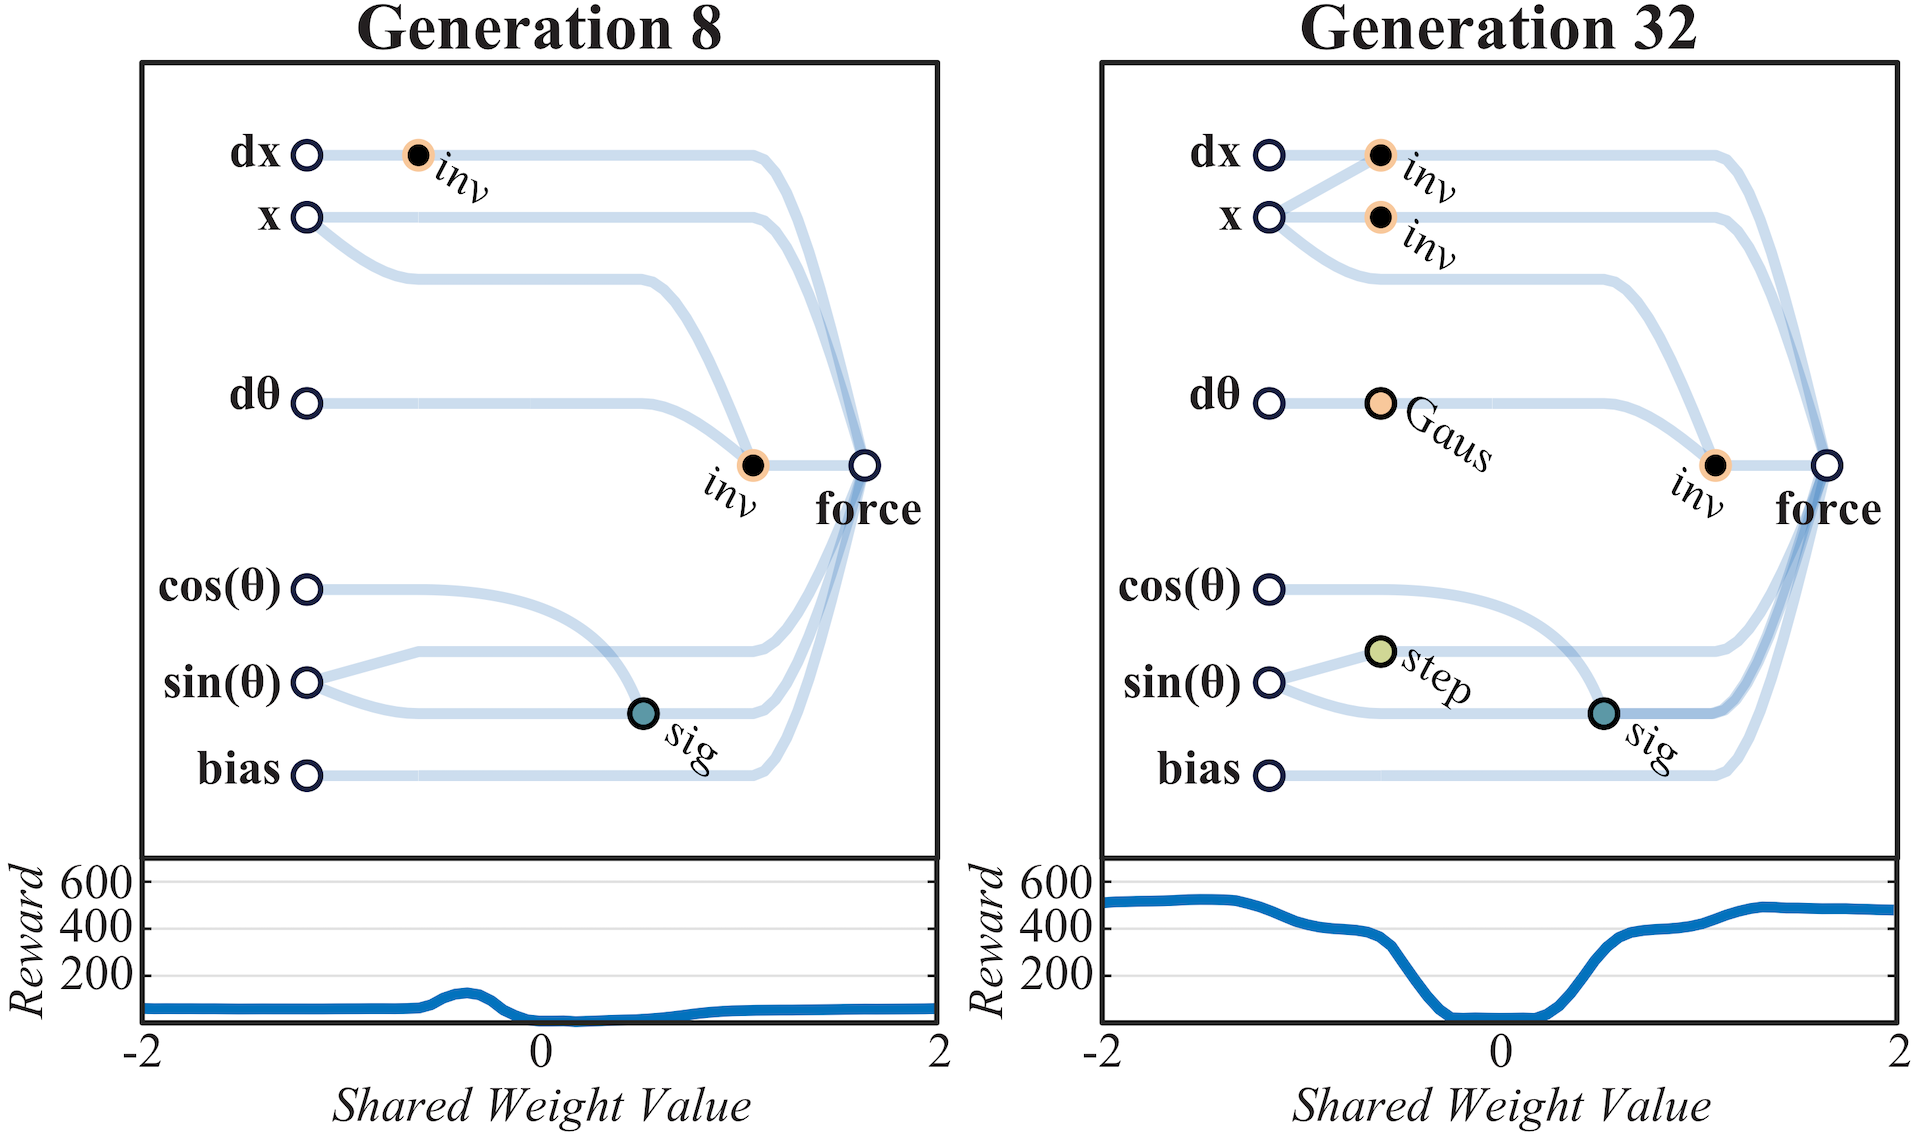
\includegraphics[width=70mm]{img/img01.png}
    \caption{共有重みと評価値とネットワーク構造}
\end{figure}

\section{提案手法}
提案手法では,慎重な活性化関数の選択を実現するために,関数同士の距離を2つの方法で求めている.1つ目は関数同士の差の積分,2つ目は関数同士のミニバッチサイズ分の入力に対する出力の差の合計を使用している.式(3)で使用されている $\varepsilon$ は式(4)に従い変動し,世代数の小さいうちは $\varepsilon$ の値は大きく擬距離関数の影響が小さくなり,世代数の大きくなると $\varepsilon$ の値は小さくなり擬距離関数を大きく考慮するようになる.変更先の関数として擬距離の近いものを選ばれやすくなるようにするのはそれまでの良い出力を反転させないようにするためだが,そもそも世代数の小さいこたいの出力は,良いものであるどころか悪いものである可能性が高い.よって,提案手法の $\varepsilon$ を最初から小さくすると悪い出力がなかなか良い方に変更されないことが懸念される.

\begin{equation}
    d(f_{a}, f_{b}) = \int^{r}_{-r} (f_{a}(x) - f_{b}(x))^{2}
\end{equation}
\begin{equation}
    d(f_{a}, f_{b}) = \sum_{m}(f_{a}(in_{m}) - f_{b}(in_{m}))^2
\end{equation}
\begin{equation}
    P_{i} =  \begin{cases} \dfrac{1}{d(f_{s}, f_{i}) + \varepsilon_{n} } \qquad (i \neq s) \\ 0 \qquad (i = s) \end{cases}\\
\end{equation}
\begin{equation}
    \varepsilon_{n} = k * \varepsilon_{n-1} \\
\end{equation}

\begin{table}[h]
    \caption{説明}
    \centering
    \begin{tabular}{cl}
        \hline
        変数  & 意味 \\
        \hline \hline
        $P_{i}$               & $s$から$i$へ活性化関数IDが変更される見込み \\
        $d(f_{s}, f_{i})$     & 活性化関数が$s$と$i$の距離                 \\
        $f_{i}$               & IDが$i$の活性化関数                        \\
        $i$                   & 活性化関数ID                               \\
        $s$                   & 現在の活性化関数ID                         \\
        $m$                   & ミニバッチサイズ x 共有重み                \\
        $in$                  & ノードに入力される値                       \\
        $\varepsilon_{n}$        & 逆数の大きさを抑えるための小さい値         \\
        $r$                   & 関数の考慮範囲                             \\
        $k$                   & $\varepsilon$の減衰率,0.995など              \\
        \hline
    \end{tabular}
\end{table}

\section{距離関数}
式(1)や式(2)の関数は,2つの活性化関数がどれだけ似ているかを示すものである.これらの関数が距離の性質を持つかどうかを示す.距離関数として満たすべき条件は以下の4つの性質である.

\begin{tabular}{cl}
    \hline
    性質  & 定義 \\
    \hline \hline
    非負性 & $d(x, y) \geq 0$ \\
    同一律 & $d(x, y) = 0 \Leftrightarrow x = y$ \\
    対称律 & $d(x, y) = d(y, x)$ \\
    三角不等式 & $d(x, y) \leq d(x, z) + d(z, y)$ \\
    \hline
\end{tabular}

同一律とは, $ x $ と $ y $ が同値であるときに限り,距離が0になるというもので, $ x $ と $ y $ が異なる値を持つ場合に距離が0になってはいけないという制約である.
式(1)における距離の性質は,上に挙げた4つの条件を満たしているが,式(2)に対しては同一律を欠くものになっている.
具体的には,ミニバッチのすべての入力(実際にタスクを解いているときのすべての入力よりとても少ないサンプル数)に限り $ f_{a}(in_{m}) = f_{b}(in_{m}) $ にさえなれば,aとbは異なる活性化関数であるにもかかわらず,距離が0となってしまう.\\
同一律の制約を緩め, $ d(x, x) = 0 $ を満たせば距離として扱ってもよいとする関数を擬距離と呼び,式(2)はこれに該当する.これは,そもそも似ている関数を選ぶ際に,頻繁に出現しない入力値を考慮せず,頻繁に出現する入力に対する出力の差が小さい関数を選びたいという糸のもと考案したものなので,同一律の満たさないことは擬距離関数の効果を疑問視する材料にはならない.

\section{進捗}
提案手法での実行をしているところ.計算量増加にともない既存手法1000世代までの実行時間と提案手法700世代までの実行時間が同じくらい.

\section{今後の目標}
卒業論文の着手

\end{document}
